\documentclass[10pt,twocolumn,letterpaper]{article}

\usepackage{cvpr}              % 使用 CVPR 风格
\usepackage[UTF8, fontset=fandol]{ctex} % 支持中文
\usepackage{newtxtext,newtxmath} % Use modern Times-like fonts
\usepackage{epsfig}
\usepackage{graphicx}
\usepackage{amsmath}
\let\Bbbk\relax
\usepackage{amssymb}
\usepackage{booktabs}
\usepackage{multirow}
\usepackage{xcolor}
\usepackage{subcaption} 

% Include other packages here, before hyperref.
% If you comment hyperref and then uncomment it, you should delete
% egpaper.aux before re-running latex.
% (Or just hit 'q' on the first latex run, let it finish, and you should be clear).
\usepackage[pagebackref=true,breaklinks=true,letterpaper=true,colorlinks,bookmarks=false]{hyperref}

% [新增] 智能引用宏包,自动处理 "Fig." "Table" 前缀
\usepackage[capitalize]{cleveref}

% Correct float placement settings
\usepackage{stfloats} 
\setcounter{dbltopnumber}{2}
\setcounter{bottomnumber}{2}
\setcounter{totalnumber}{4}
\renewcommand{\dbltopfraction}{0.9}
\renewcommand{\bottomfraction}{0.8}
\renewcommand{\textfraction}{0.07}

% \cvprfinalcopy % *** Uncomment this line for the final submission
\def\cvprPaperID{****} % *** Enter the Paper ID here

\def\httilde{\mbox{\tt\raisebox{-.5ex}{\symbol{126}}}}

% Pages are numbered in submission mode, and unnumbered in camera-ready
\ifcvprfinal\pagestyle{empty}\fi

\begin{document}

%%%%%%%%% TITLE
\title{结构感知的视觉-语言对齐:\\ 用于密集视频定位的掩膜先验引导注意力机制}

\author{Your Name\\
Institution Name\\
{\tt\small first.author@i1.org}
% For a paper whose authors are all at the same institution,
% omit the following lines up until the closing ``}''.
% Additional authors and addresses can be added with ``\and'',
% just like the second author.
% To save space, use either the email address or home page, not both
\and
Second Author\\
Institution2\\
{\tt\small second.author@i2.org}
}

\maketitle
%\thispagestyle{empty}

%%%%%%%%% ABSTRACT
\begin{abstract}
多模态大语言模型(MLLM)在通用视觉理解方面展现了卓越的能力。
然而,在像素级密集预测任务中,例如指代视频对象分割(RVOS),这些模型通常受到注意力幻觉(即模型关注背景噪声而非特定目标)以及粗糙边界描绘的困扰。
为了弥补这一差距,我们提出了一个\textbf{结构感知的视觉-语言对齐}框架。
我们的方法引入了一种\textbf{掩膜偏置注意力}机制,利用低级视觉特征作为显式空间先验来门控跨模态注意力,从而有效抑制不相关区域。
此外,我们设计了一种\textbf{细粒度语义-结构对齐}策略,结合了文本-掩膜对比(TMC)损失和边界一致性约束,以确保高层语言语义与像素级细节之间的精确对齐。
在多个基准测试上的广泛实验表明,我们的方法达到了最先进的性能。
值得注意的是,在 DAVIS 2017 视频分割基准(val)上,我们的模型达到了 \textbf{71.9\% J\&F}(比 Sa2VA-1B 基线高出 3.4\%),同时在复杂运动理解任务(MeVis)上保持了鲁棒的性能,验证了我们结构先验的精确性和泛化能力。
代码将在 https://github.com/pengrui-art/MPR-CMA 开源。
\end{abstract}

%%%%%%%%% BODY TEXT
\section{引言}

大语言模型(LLM)与视觉基础模型的融合催生了从专用分割网络向统一的多模态大语言模型(MLLM)的范式转变。
像 \textbf{Sa2VA} \cite{sa2va} 和 \textbf{LIRA} \cite{lira} 这样的旗舰框架已成功将 LLM(例如 Qwen \cite{qwenvlplus}, InternVL \cite{internvl25})的推理能力与 \textbf{SAM-2} \cite{sam2} 的像素级精度集成在一起。
这些统一模型在零样本性能上表现出色,理论上实现了跨图像和视频的通用定位(Grounding)与分割能力。

\begin{figure}[h!]
    \centering
    \setlength{\abovecaptionskip}{5pt}
    \setlength{\belowcaptionskip}{-5pt}
    
    % --- Row 1: Relative Position ---
    \begin{subfigure}[t]{0.32\linewidth}
        \centering
        \scriptsize \textbf{输入图像} \par \medskip
        
\includegraphics[width=1\linewidth]{figures/cup.jpg}
    \end{subfigure}
    \hfill
    \begin{subfigure}[t]{0.32\linewidth}
        \centering
        \scriptsize \textbf{OMG-LLaVA} \par \medskip
        \includegraphics[width=1\linewidth]{figures/cup_llava.jpg}
    \end{subfigure}
    \hfill
    \begin{subfigure}[t]{0.32\linewidth}
        \centering
        \scriptsize \textbf{Ours} \par \medskip
        \includegraphics[width=1\linewidth]{figures/cup_sa2va.jpg}
    \end{subfigure}
    
    \vspace{1mm}
    \begin{minipage}{0.98\linewidth}
        \centering
        \scriptsize \textit{“分割笔记本电脑\textbf{后面}的马克杯。”}
    \end{minipage}
    
    \vspace{1mm}

    % --- Row 2: Spatial Ordering ---
    \begin{subfigure}[t]{0.32\linewidth}
        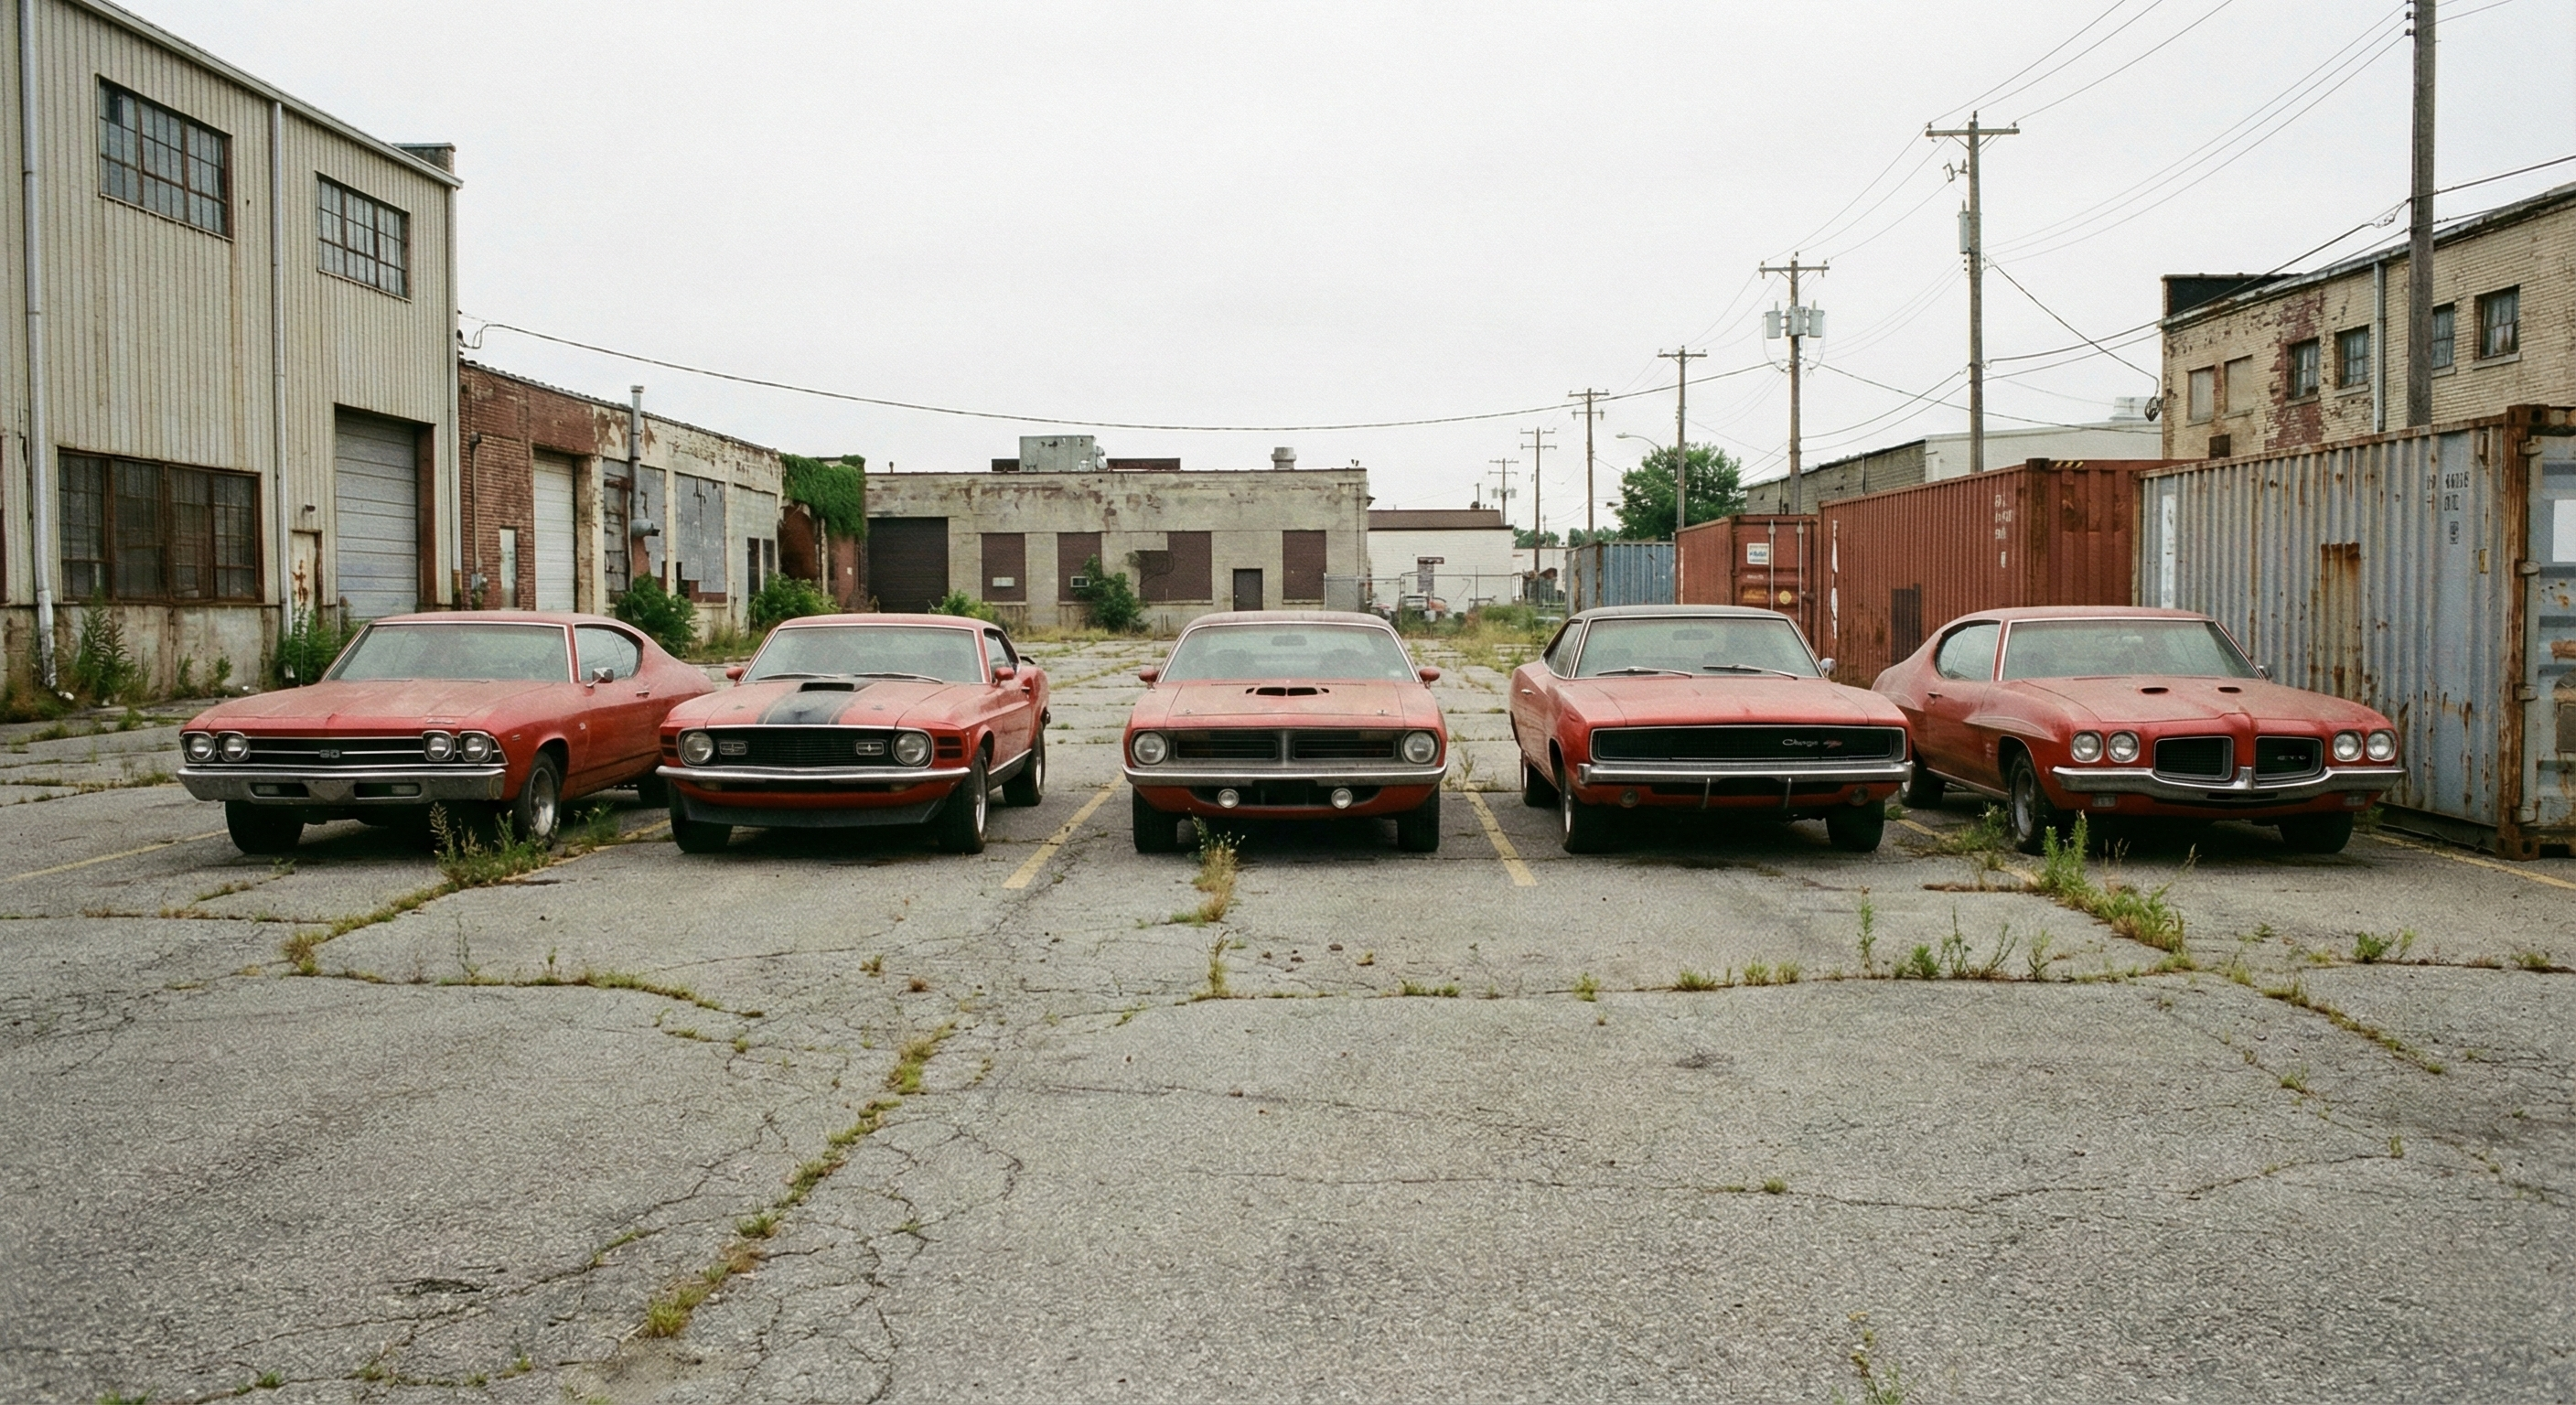
\includegraphics[width=1\linewidth]{figures/car.jpg}
    \end{subfigure}
    \hfill
    \begin{subfigure}[t]{0.32\linewidth}
        \includegraphics[width=1\linewidth]{figures/car_llava.jpg}
    \end{subfigure}
    \hfill
    \begin{subfigure}[t]{0.32\linewidth}
        \includegraphics[width=1\linewidth]{figures/car_sa2va.jpg}
    \end{subfigure}
    
    \vspace{1mm}
    \begin{minipage}{0.98\linewidth}
        \centering
        \scriptsize \textit{“分割从右边数的\textbf{第二辆}红色汽车。”}
    \end{minipage}
    
    \vspace{1mm}

    % --- Row 3: Interaction ---
    \begin{subfigure}[t]{0.32\linewidth}
        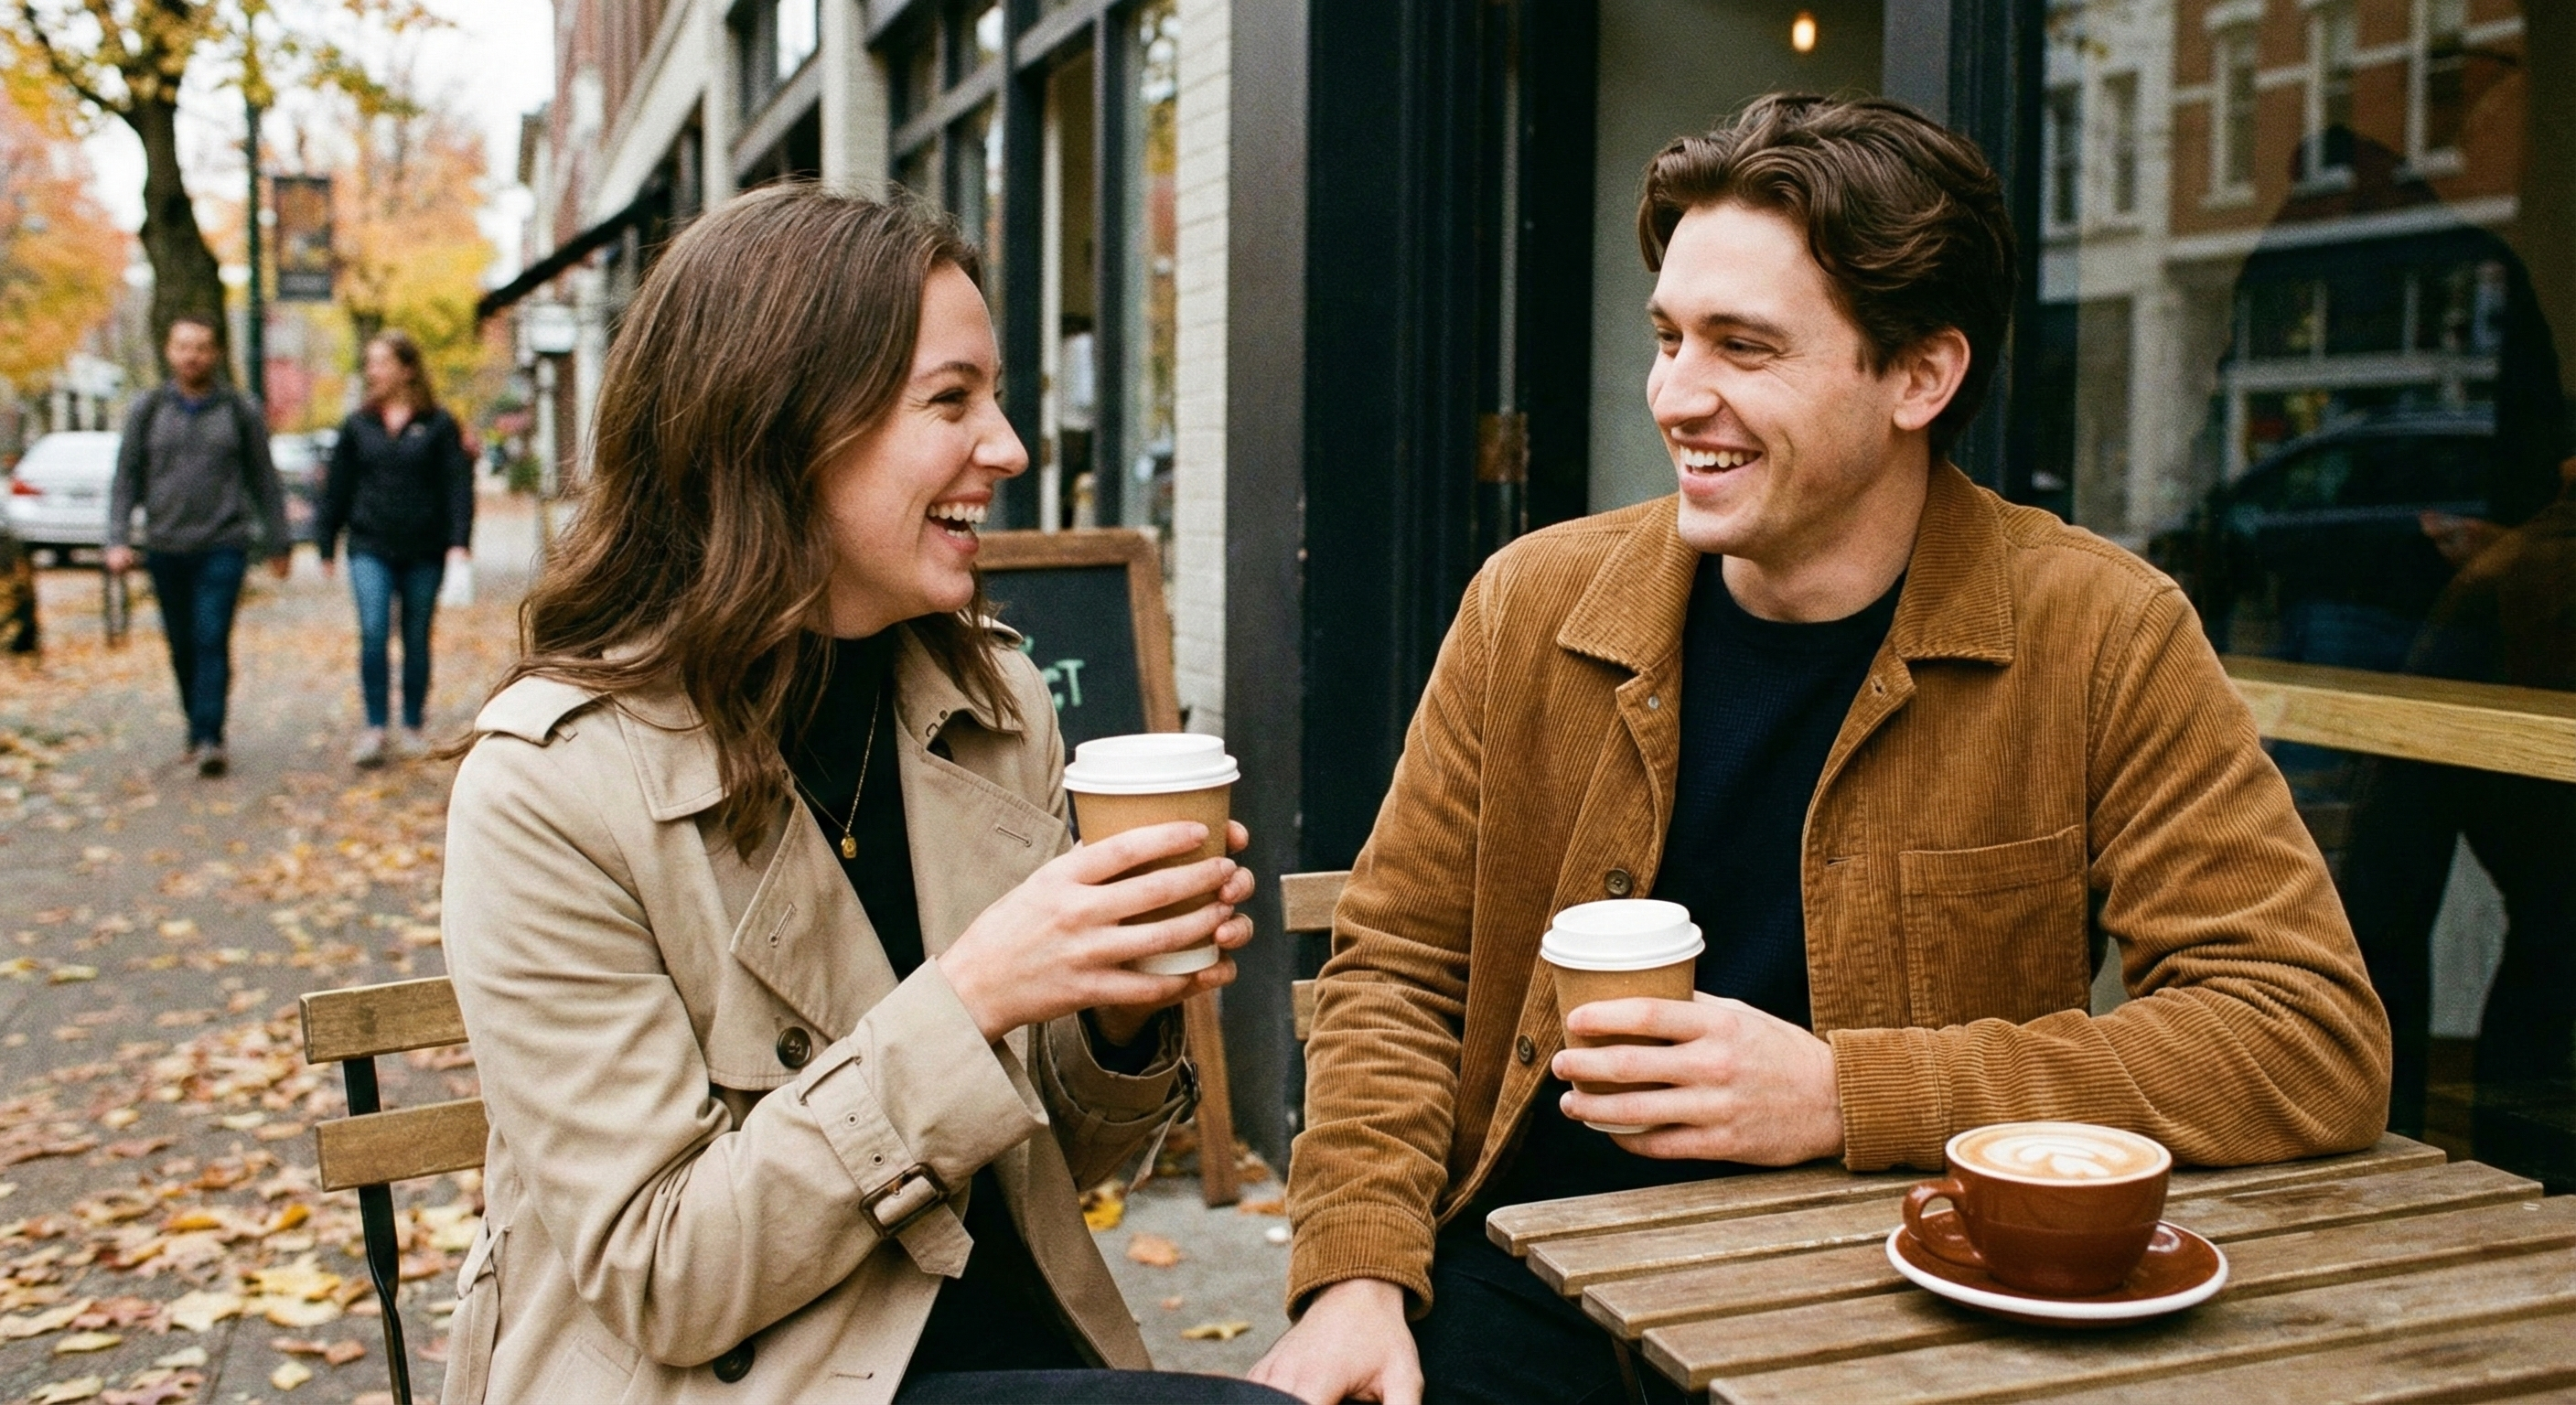
\includegraphics[width=1\linewidth]{figures/coffee.jpg}
    \end{subfigure}
    \hfill
    \begin{subfigure}[t]{0.32\linewidth}
        \includegraphics[width=1\linewidth]{figures/coffee_llava.jpg}
    \end{subfigure}
    \hfill
    \begin{subfigure}[t]{0.32\linewidth}
        \includegraphics[width=1\linewidth]{figures/coffee_sa2va.jpg}
    \end{subfigure}

    \vspace{1mm}
    \begin{minipage}{0.98\linewidth}
        \centering
        \scriptsize \textit{“分割穿白衣服的人\textbf{拿着的}杯子。”}
    \end{minipage}

    \vspace{0.3cm}
    \caption{\textbf{解决注意力幻觉。} 
    与遭受注意力漂移的 OMG-LLaVA(中)不同,我们的结构感知 Sa2VA(右)明确注入了结构先验,以精确地定位由复杂空间约束(例如,深度、排序、交互)定义的对象。}
    \label{fig:teaser}
\end{figure}

然而,一个关键的\textbf{语义-结构差距}尚未解决。
虽然当前的 MLLM 擅长高层语义对齐,但在细粒度结构对齐方面却表现出明显的性能下降。
我们观察到,像 Sa2VA 和 \textbf{GLaMM} \cite{glamm} 这样的模型将视觉特征视为抽象的语义 Token,剥离了描绘边界所必需的低级空间先验。
这导致了\textbf{注意力幻觉}:如 \Cref{fig:teaser} 所示,当面对复杂的空间查询(例如,“\textit{笔记本电脑后面的杯子}”)时,跨模态注意力图会漂移向最显著的物体,而不是空间关系定义的目标。
因此,尽管使用了 SAM-2 的解码器,但在像 MeVis 这样的复杂基准测试上的定位质量仍落后于人类表现,J\&F 通常停滞在 46.9\% 左右。
为了弥补这一差距,我们引入了 \textbf{Structure-Aware Sa2VA(结构感知 Sa2VA)},该框架在 MLLM 注意力机制内强制执行结构保真度。
与依赖显式视觉提示(点/框)的 \textbf{SegGPT} 或 \textbf{SEEM},以及通过交错训练隐式学习对齐的 \textbf{LIRA} 不同,我们的方法直接将显式的 \textbf{掩膜偏置注意力 (MBA)} 先验注入到 Transformer 层中。
通过利用源自视觉主干的低级结构线索来调制 LLM 的注意力权重,我们抑制了背景噪声并锁定目标对象的拓扑结构。
我们的贡献总结如下:
\begin{itemize}
    \item \textbf{结构感知注意力机制。} 我们提出了一种\textbf{掩膜偏置注意力 (MBA)},这是一种轻量级的空间门控模块,显式地将掩膜先验注入跨模态交互中。这通过锁定目标的拓扑结构,有效抑制了注意力幻觉(第~\ref{sec:mba}节)。
    \item \textbf{细粒度双重对齐。} 我们引入了一种由\textbf{文本-掩膜对比 (TMC)} 学习和\textbf{边界一致性约束}监督的细粒度对齐策略。这些目标强制执行语言语义与像素级结构细节之间的精确同步(第~\ref{sec:alignment}节)。
    \item \textbf{最先进的性能。} 广泛的实验表明,我们的方法显著优于 Sa2VA 基线和其他 MLLM。值得注意的是,我们在 DAVIS 2017 上达到了 \textbf{71.9\% J\&F} (+3.4\%),并在 RefCOCOg 上展现了卓越的复杂推理能力,验证了我们结构先验的有效性。至关重要的是,我们保留了InternVL的开放式对话能力,而没有出现微调专用模型中常见的显着性能下降。
\end{itemize}

%-------------------------------------------------------------------------
\section{相关工作}

\subsection{统一多模态分割}
该领域已从专用模型迅速发展为统一的通用模型。
像 \textbf{LISA} \cite{lisa} 和 PixelLM 这样的早期尝试引入了 \texttt{[SEG]} Token 范式,将语言嵌入映射到静态掩码。
\textbf{GLaMM} \cite{glamm} 将其扩展到像素定位,但在时间一致性方面存在困难。
最先进的 \textbf{Sa2VA} \cite{sa2va} 通过将 \textbf{SAM-2} \cite{sam2} 与 InternVL2 集成,将图像和视频任务统一起来,将视频帧视为连续的视觉 Token。
虽然 Sa2VA 实现了强大的基线(DAVIS 上 75.2\% J\&F),但它缺乏明确的机制来约束注意力,导致在拥挤场景中出现“对象漂移”。
同样,\textbf{LIRA} \cite{lira} 提出了交错局部视觉耦合 (ILVC) 以减少幻觉,但其依赖隐式回归通常无法在复杂运动场景中保持清晰的边界。
我们的工作通过将结构先验直接注入注意力机制来明确纠正这一点。

\subsection{通用和交互式分割}
像 \textbf{SAM-2} \cite{sam2}、SEEM 和 SegGPT 这样的基础视觉模型已经解决了基于提示(点、框)输入的“分割一切”任务。
例如,SAM-2 在提供预言机(Oracle)视觉提示时,在 DAVIS 上达到了 90.7\% 的 J\&F。然而,这些模型是\textbf{语义盲}的;
它们无法对开放词汇文本查询(例如,“\textit{正在跑步的人}”)进行推理。
相反,像 \textbf{OpenSeeD} 和 \textbf{CutLER} 这样的开放词汇方法处理检测,但缺乏视频所需的像素级跟踪一致性。
\textbf{Sa2VA} 弥合了这一鸿沟:利用 MLLM 的语义推理来生成指导 SAM-2 解码器结构精度的“提示”,有效地自动化了原始 SAM-2 中人机交互的需求。

\subsection{现有技术中的结构引导对齐}
先前的工作试图通过外部模块强制执行结构。
\textbf{Osprey} 和 \textbf{OMG-LLaVA} \cite{omgllava} 使用掩码池化或以对象为中心的 Token 来表示区域。
然而,这些方法通常将空间细节压缩成一维 Token,丢失了细粒度的拓扑结构。
\textbf{PSALM} \cite{psalm} 引入了掩码 Token,但仅限于静态图像。
与将几何编码为文本的 Structure-LLM 不同,我们的 \textbf{掩膜偏置注意力} 在连续特征空间中运行,动态调制注意力图。
这确保了对“左”、“后”或“接触”的语言理解是物理地建立在视觉特征图之上,而非由语言模型幻觉产生的。

%-------------------------------------------------------------------------
\section{方法论}
我们提出的结构感知 Sa2VA 的整体流程如 \Cref{fig:framework} 所示。
该框架由三个集成阶段组成:
(1) \textbf{共享视觉编码器:} 视觉编码器和 LLM 处理输入视频和文本,提取多尺度视觉特征和文本嵌入。
(2) \textbf{掩膜偏置注意力:} 提出的 MBA 机制将来自 SAM-2 解码器的像素级结构先验注入跨模态交互中,以防止注意力漂移。
(3) \textbf{细粒度对齐:} 最后,模型通过涉及文本-掩膜对比(TMC)损失和边界一致性损失的双重约束策略进行监督,以确保高保真分割。

\begin{figure*}[t]
    \centering
    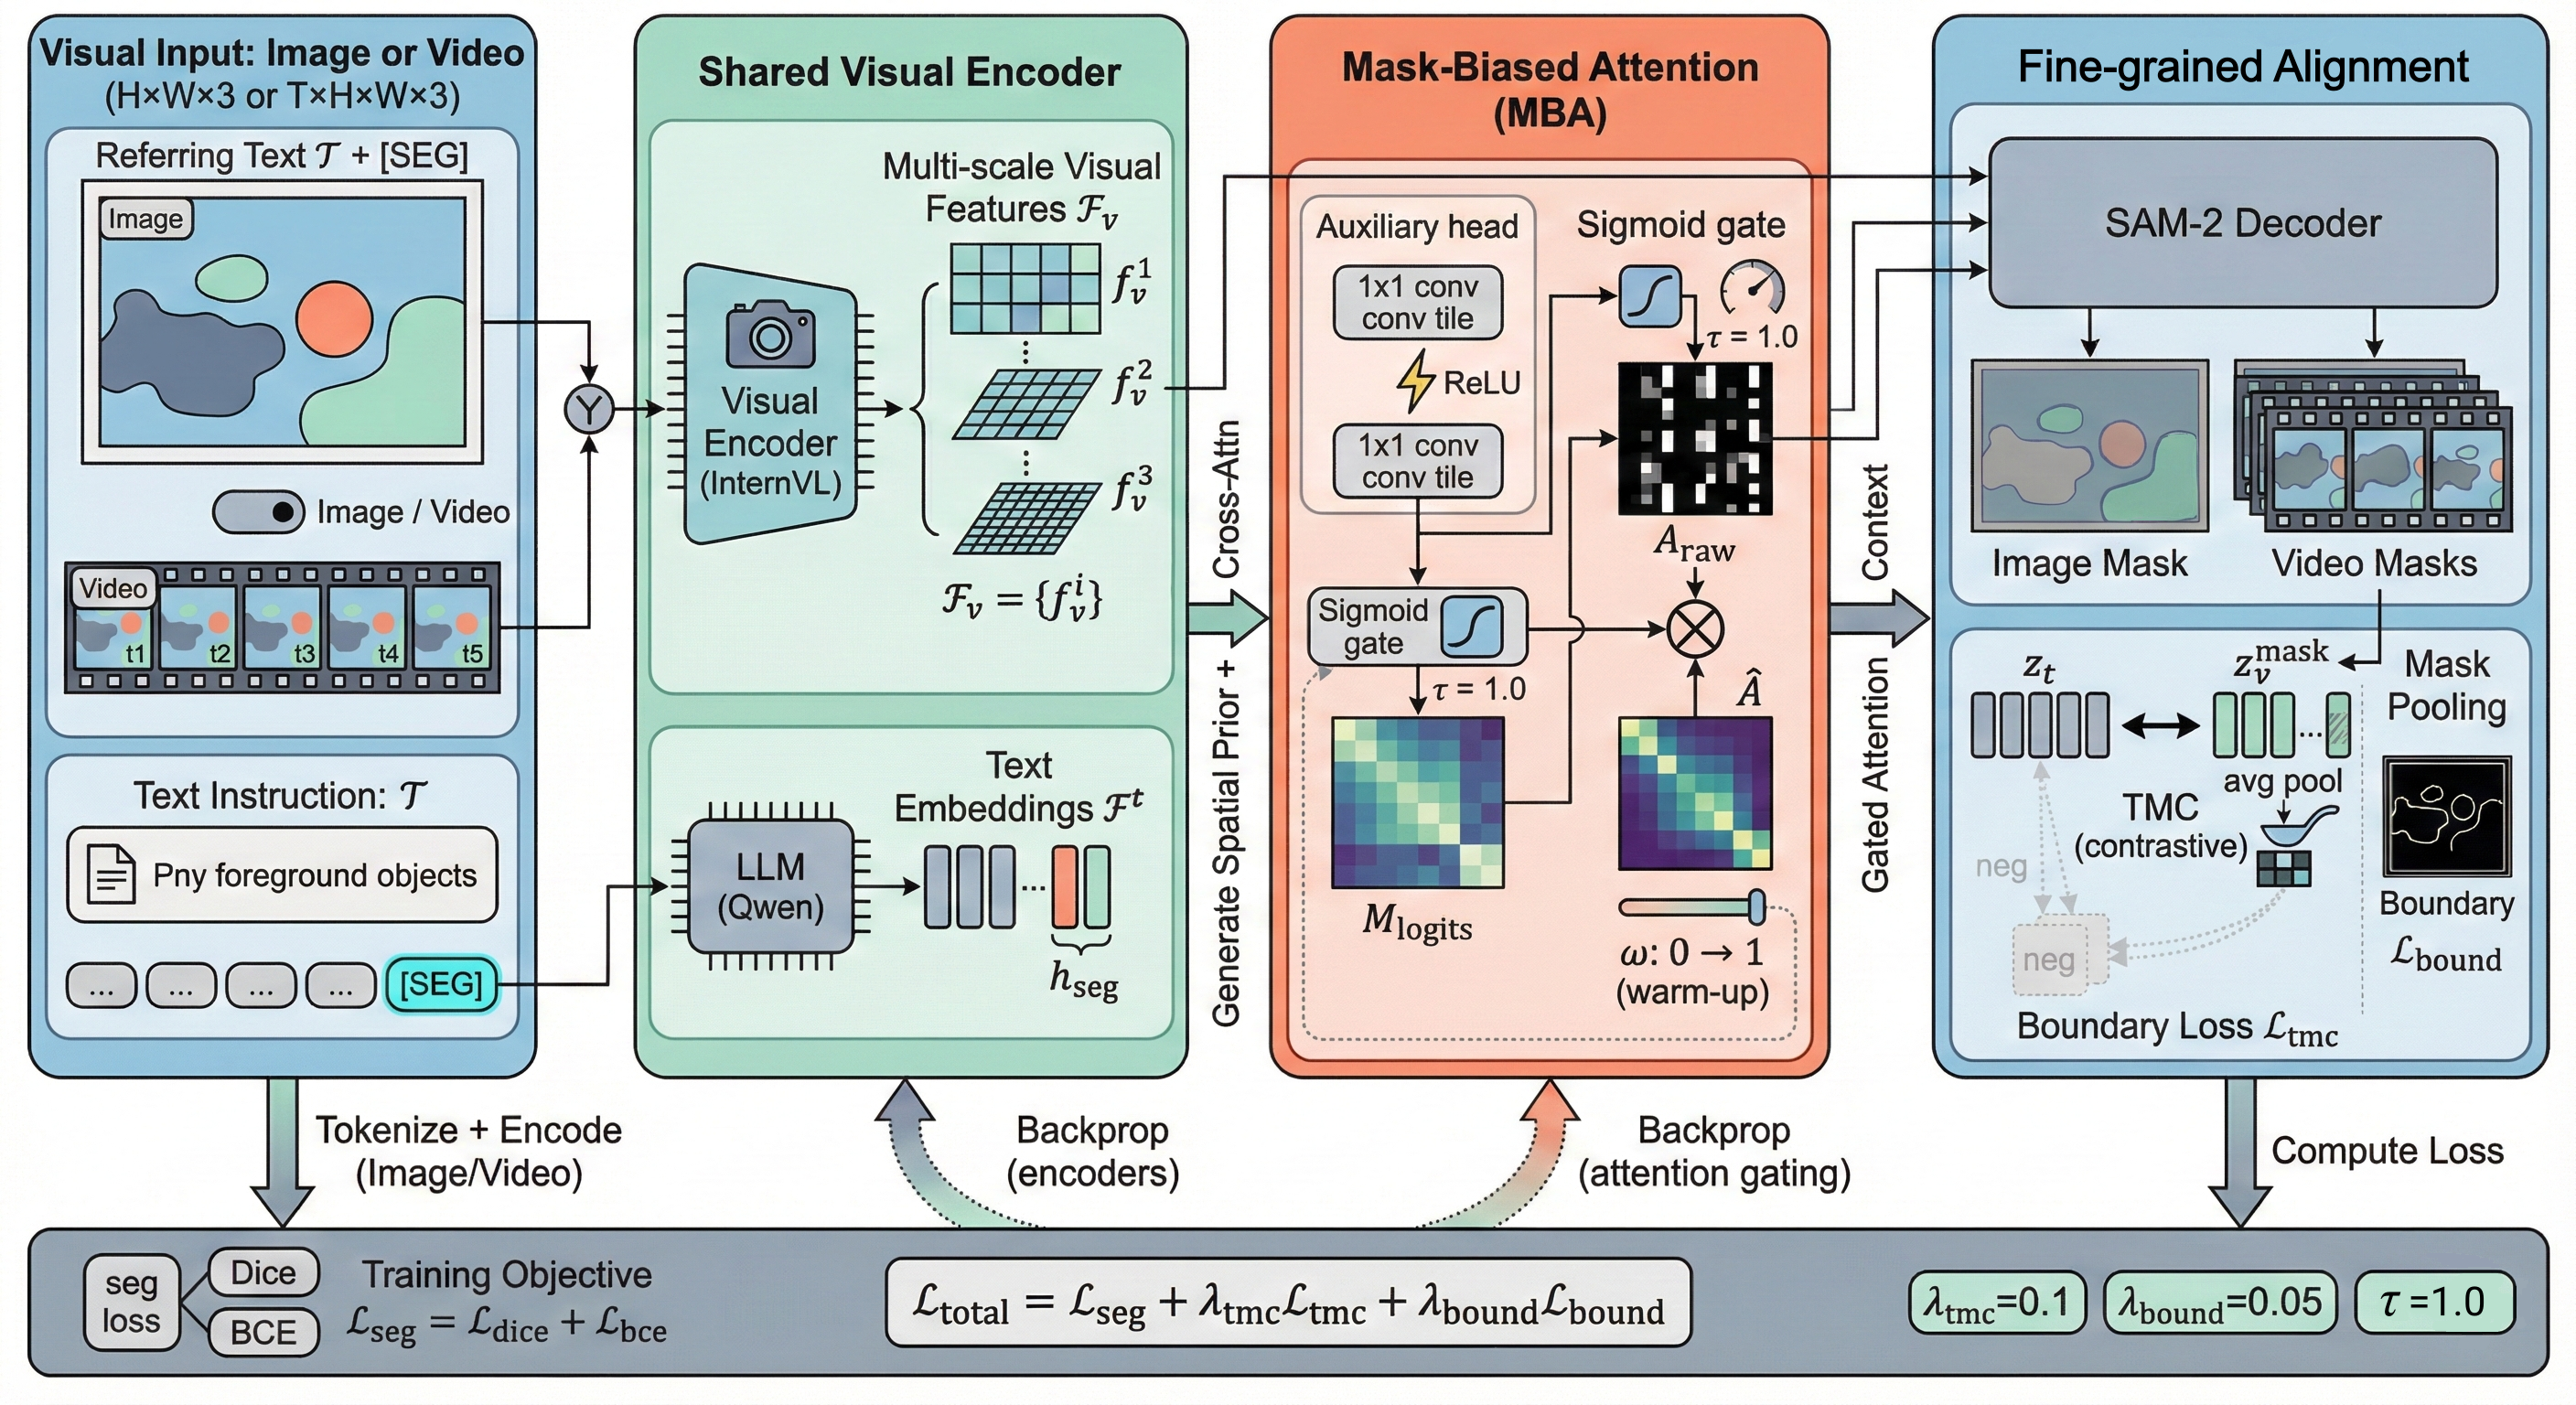
\includegraphics[width=1.0\linewidth]{figures/framework_overview.jpg}
    \caption{\textbf{框架概览。} \textbf{(a) 共享视觉编码器。} 提取多尺度视觉特征 $\mathcal{F}_v$ 和文本嵌入。
    \textbf{(b) 掩膜偏置注意力。} 辅助头生成低分辨率先验 $M_{prior}$,该先验通过 Sigmoid 转换为空间门 $G$。
    该门与交叉注意力图相乘 ($\otimes$) 以抑制噪声。
    \textbf{(c) 细粒度对齐。} 我们通过文本-掩膜对比 (TMC) 损失 ($\leftrightarrow$) 强制执行语义对齐,并通过边界损失(突出显示的轮廓)强制执行结构精度。}
    \label{fig:framework}
\end{figure*}

\subsection{问题阐述}
\label{sec:preliminaries}

% [Part 1: 确立地位 - Authority & Foundation]
我们的框架建立在 \textbf{Sa2VA}~\cite{sa2va} 之上,它代表了当前用于密集定位的统一多模态大语言模型 (MLLM) 的最先进水平。
与以前的专用模型(例如用于图像的 LISA~\cite{lisa} 或 MeViS 专用基线)不同,Sa2VA 无缝集成了 \textbf{InternVL-2} 的语义推理能力与 \textbf{SAM-2}~\cite{sam2} 强大的分割解码能力。
我们选择 Sa2VA 作为基础,因为它理论上提供了两全其美的优势:LLM 的开放式泛化能力和基础视觉模型的掩码质量。

% [Part 2: 诊断病灶 - The Problem Hierarchy]
然而,我们发现了该架构固有的一个关键\textbf{结构瓶颈}。
虽然 Sa2VA 擅长高层语义识别(例如,识别“一只狗”),但在处理细粒度空间指令时,它会出现不同程度的退化:
\begin{itemize}
    \item \textbf{语义对齐:} 模型有效地将文本与不同对象的视觉区域对齐。然而,\texttt{[SEG]} Token 的隐式注入通常导致在对象共享相似语义属性时定位粗糙。
    \item \textbf{结构幻觉:} 如第 1 节所述,严重的限制出现在复杂推理场景中(例如,相对定位或严重遮挡)。由于 Sa2VA 将视频帧视为抽象的一维语义 Token,它剥离了精确边界描绘所需的低级 2D/3D 空间几何信息。在没有显式空间约束的情况下,跨模态注意力机制表现出\textbf{注意力漂移},即模型幻觉般地关注背景噪声或相邻的干扰项,而不是目标的拓扑结构。
\end{itemize}

% [Part 3: 承上启下 - Motivation]
这一诊断表明,简单地扩展数据或参数无法解决结构缺陷。
相反,它需要一种显式机制将空间先验重新引入 MLLM 的推理过程,这激发了我们提出的 \textbf{掩膜偏置注意力 (Mask-Biased Attention)}。

\subsection{掩膜偏置注意力}
\label{sec:mba} 
标准方法通常允许视觉特征与所有文本 Key 进行交互,而没有结构约束。
我们提出,视觉特征应该主动“查询”相关的文本信息,但这一过程必须经过空间门控,以防止背景噪声吸收不相关的语义上下文。

\textbf{来自 SAM-2 解码器的空间先验。}
我们不引入单独的轻量级分支,而是利用预训练 SAM-2 解码器强大的掩码预测能力。
我们利用 SAM-2 掩码解码器生成的中间掩码 logits $M_{logits}$ 作为我们的空间先验。
这确保了注意力机制由当前迭代中可用的最准确的结构估计来引导。

\begin{figure}[h]
    \centering
    \includegraphics[width=1.0\linewidth]{figures/mechanism.jpg}
    \caption{\textbf{掩膜偏置注意力机制。} 
    该模块利用学习到的空间先验 $G$(中)来门控交叉注意力的输出。
    通过应用逐元素乘法 $\otimes$,注入的文本语义被严格限制在目标对象上。}
    \label{fig:mba_module}
\end{figure}

\textbf{带有 Top-K 路由的视觉-查询注意力。}
与标准实现(全局文本嵌入查询视觉特征)相反,我们反转了交互方向。
设 $\mathcal{F}_v \in \mathbb{R}^{HW \times C}$ 表示展平的视觉特征图,$\mathcal{F}_t = \{t_1, \dots, t_N\} \in \mathbb{R}^{N \times C}$ 为 $N$ 个文本 Token 的序列。
我们将视觉特征定义为查询 ($Q = \mathcal{F}_v$),将文本 Token 定义为键 ($K$) 和值 ($V$)。
这种像素到文本的公式允许每个空间位置检索特定的细粒度语义细节。
为了提高计算效率,我们采用了 \textbf{Top-K Token 路由}策略。
我们使用轻量级 MLP 路由器为每个文本 Token 计算标量重要性分数 $s_i$:
\begin{equation}
    s_i = \text{MLP}(t_i).
\end{equation}
然后,我们选择前 $K$ 个最相关的 Token 子集 $\hat{\mathcal{F}}_t = \{t_i \mid i \in \text{TopK}(s)\}$ 作为键-值对。
检索到的语义特征 $\mathcal{O}_{attn}$ 通过标准多头注意力 (MHA) 计算:
\begin{equation}
    \mathcal{O}_{attn} = \text{MHA}(Q=\mathcal{F}_v, K=\hat{\mathcal{F}}_t, V=\hat{\mathcal{F}}_t).
\end{equation}

\textbf{掩膜门控输出调制。}
我们不是隐式地偏置注意力权重,而是利用来自 SAM-2 解码器的结构先验显式地调制输出,如 \Cref{fig:mba_module} 所示。
我们首先使用温度缩放的 Sigmoid 函数将掩码 logits $M_{logits} \in \mathbb{R}^{H \times W}$ 归一化为软空间门 $G$:
\begin{equation}
    G_{i,j} = \sigma\left(\frac{M_{logits}^{(i,j)}}{\tau_{gate}}\right),
\end{equation}
其中 $\tau_{gate}$ 控制结构先验的锐度。
最后,文本感知特征通过门控残差连接注入到视觉主干中:
\begin{equation}
    \mathcal{F}_{v}' = \mathcal{F}_v + \gamma \cdot (\mathcal{O}_{attn} \odot G),
\end{equation}
其中 $\odot$ 表示跨通道维度广播的逐元素乘法,$\gamma$ 是初始化为 0 的可学习缩放因子。
这种门控机制有效地抑制了文本语义注入到背景区域,确保 VLM 的推理严格限制在感兴趣的对象上。

\textbf{残差预热策略。}
为了确保训练稳定性,我们对可学习的残差门控因子 $\gamma$ 应用线性预热。
它从接近零开始并逐渐增加,允许模型在不破坏初始特征学习的情况下缓慢整合结构感知引导。

\subsection{细粒度对齐}
\label{sec:alignment}

% [新增] Motivation 段落 - 解释为什么要加 TMC 和 Boundary Loss
虽然掩膜偏置注意力机制成功地在特征层面注入了空间先验,但仅依靠这种交互对于高精度分割来说是不够的。
我们观察到,如果没有针对细粒度细节的显式监督信号,模型仍可能收敛到次优解,即视觉特征漂移向语义相似但空间上不同的实例(例如,合并两辆相邻的“红色汽车”)。
这需要双重约束策略,在优化阶段明确强制执行高层语言语义与像素级结构边界之间的对齐。

% [原有内容的自然衔接]
为此,我们引入了双重约束对齐策略,如 \Cref{fig:framework} \textbf{右侧}所示。

\textbf{文本-掩膜对比学习。}
为了防止视觉特征在解码过程中偏离文本指令,我们强制执行语义一致性约束。
具体来说,我们通过在预测的前景区域 $\mathcal{M}$ 上对特征图 $\mathcal{F}_v$ 进行平均池化来提取区域级视觉特征 $z_v^{mask}$。
设 $z_t$ 为指令的句子级嵌入。
我们采用对称 InfoNCE 损失来最大化匹配的文本-视觉对 $(z_t, z_v^{mask})$ 之间的互信息:
\begin{equation}
    \mathcal{L}_{tmc} = \mathcal{L}_{v \to t} + \mathcal{L}_{t \to v}
\end{equation}
其中两个方向(视觉到文本和文本到视觉)均由温度 $\tau_{tmc}$ 归一化。
该对称目标显式地将“关注区域”的潜在空间与语言指令对齐,确保模型不仅关注正确的位置,还能理解正确的语义。

\textbf{边界一致性约束。}
标准的二元交叉熵 (BCE) 和 Dice 损失主要关注整体掩码区域,但对边界误差不敏感。
然而,在视频分割中,模糊的边界是质量下降的主要来源(例如,时间抖动)。
我们结合了边界损失 $\mathcal{L}_{bound}$ 来惩罚预测边界轮廓与真实边缘之间的分布距离。
通过优化特定的高频结构误差,该项充当输出掩码的细粒度锐化器。

\subsection{统一训练目标}

% [新增] Motivation 段落 - 解释 Loss 组合的逻辑
一个鲁棒的视频定位框架必须平衡两个相互竞争的目标:全局语义保真度(理解“是什么”和“在哪里”)和局部结构精度(描绘“具体如何”)。
仅靠标准分割损失通常无法捕捉这种平衡,导致掩码虽然语义正确但结构粗糙。
因此,我们制定了一个统一的优化目标,将通用分割监督与我们提出的结构感知约束线性结合起来。

% [原有公式部分]
我们的总损失函数定义为:
\begin{equation}
    \mathcal{L}_{total} = \mathcal{L}_{seg} + \lambda_{tmc}\,\mathcal{L}_{tmc} + \lambda_{bound}\,\mathcal{L}_{bound}
\end{equation}

其中:
\begin{itemize}
    \item $\mathcal{L}_{seg} = \mathcal{L}_{dice} + \mathcal{L}_{bce}$:这是 SAM-2 中使用的 Dice 损失和二元交叉熵损失的标准线性组合,负责通用掩码质量。
    \item $\mathcal{L}_{tmc}$:文本-掩膜对比损失 (\Cref{sec:alignment}) 强制执行语义保真度。
    \item $\mathcal{L}_{bound}$:边界损失 (\Cref{sec:alignment}) 强制执行高频结构精度。
\end{itemize}

\textbf{超参数选择。}
我们根据经验将平衡系数设置为 $\lambda_{tmc}=0.1$ 和 $\lambda_{bound}=0.05$。
我们观察到边界损失梯度通常比语义损失更明显;
因此,较低的权重可防止其压倒优化稳定性。

%-------------------------------------------------------------------------
\section{实验}

\subsection{实施细节}
我们采用 1B 参数版本的 Sa2VA 作为我们的基线框架。
模型使用 AdamW 进行优化,学习率为 $4 \times 10^{-5}$,权重衰减为 $0.05$。
对于损失平衡系数,我们根据经验设置 $\lambda_{tmc}=0.1$ 和 $\lambda_{bound}=0.05$,以平衡语义对齐和结构精度,而不会破坏训练稳定性。
掩模偏置温度 $\tau_{gate}$ 设置为 1.0,对比温度 $\tau_{tmc}$ 设置为 0.15。
所有实验均在 4 $\times$ NVIDIA RTX 5090 (32GB) GPUs 上进行。
训练过程运行 1 个 epoch,在最初 5\% 的迭代中使用线性预热阶段,以提高辅助损失和 MBA 门控因子的影响。

\subsection{数据集设置}
我们在三个不同类别的基准测试上评估了我们结构感知框架的有效性,以确保全面的分析:
\begin{itemize}
    \item \textbf{图像指代分割:} 我们使用 \textbf{RefCOCO}, \textbf{RefCOCO+} 和 \textbf{RefCOCOg} 数据集。
    这些数据集要求模型在静态图像中分割由自然语言查询描述的特定对象。
    \item \textbf{视频对象分割 (VOS):} 我们使用 \textbf{DAVIS 2017}。该基准强调对象掩膜的像素级质量和时间一致性,作为我们模型结构感知能力的主要指标。
    \item \textbf{指代视频对象分割 (R-VOS):} 我们使用 \textbf{MeVis}。与 DAVIS 不同,这些数据集(尤其是 MeVis)专注于复杂的运动表达(例如,“飞走的那只鸟”),测试模型理解动态动作而不仅仅是静态外观的能力。
\end{itemize}

\subsection{与最先进技术的比较}
我们提供了我们的方法 (Sa2VA-Structure) 与领先的多模态大语言模型 (MLLM) 的全面比较。
如 \Cref{tab:sota_comparison} 所示,我们评估了三个不同维度的性能:图像指代分割(RefCOCO 系列)、视频分割(DAVIS、MeVis)和通用多模态理解 (MME, MMBench, SEED)。

\begin{table*}[t]
    \centering
    \caption{\textbf{与最先进方法的比较。} 我们报告图像指代分割任务的 cIoU,视频分割任务的 $\mathcal{J}\&\mathcal{F}$,以及多模态理解的标准指标。
    最好的结果以\textbf{粗体}突出显示。结构感知 Sa2VA 在视频分割任务和复杂指代场景(例如 RefCOCOg)上取得了最先进的性能,同时保持了有竞争力的通用理解能力。}
    \label{tab:sota_comparison}
    \renewcommand{\arraystretch}{1.1}
    \resizebox{\textwidth}{!}{
    \begin{tabular}{l|ccc|ccc|cc|cc|ccc}
        \toprule
        \multirow{3}{*}{\textbf{Method}} & \multicolumn{8}{c|}{\textbf{图像分割}} & \multicolumn{2}{c|}{\textbf{视频分割}} & \multicolumn{3}{c}{\textbf{图像对话}} \\
         & \multicolumn{3}{c|}{RefCOCO} & \multicolumn{3}{c|}{RefCOCO+} & \multicolumn{2}{c|}{RefCOCOg} & \multirow{2}{*}{DAVIS} & \multirow{2}{*}{MeVis} & \multirow{2}{*}{MME} & \multirow{2}{*}{MMB} & \multirow{2}{*}{SEED} \\
        & Val & TestA & TestB & Val & TestA & TestB & Val & Test & & & & & \\
        \midrule
        LLAVA-1.5-13B & - & - & - & - & - & - & - & - & - & - & 1531(+) & 68.8 & 70.1 \\
        Video-LLaVA-7B & - & - & - & - & - & - & - & - & - & - & - & 60.9 & - \\
        LLaMA-VID-7B & - & - & - & - & - & - & - & - & - & - & 1521(+) & 65.1 & 59.9 \\
        mPLUG-Owl3-8B & - & - & - & - & - & - & - & - & - & - & - & 77.6 & - \\
        InternVL2-8B & - & - & - & - & - & - & - & - & - & - & - & 81.7 & 76.2 \\
        PixelLM-7B & 73.0 & - & - & 66.3 & - & - & 69.3 & - & - & - & 309/135 & 17.4 & - \\
        PixelLM-13B \cite{pixellm} & 73.0 & 76.5 & 68.2 & 66.3 & 71.7 & 58.3 & 69.3 & 70.5 & - & - & 309/135 & 17.4 & - \\
        LaSagnA & 76.8 & - & - & 66.4 & - & - & 70.6 & - & - & - & 0/0 & 0.0 & - \\
        LISA-7B \cite{lisa} & 74.1 & 76.5 & 71.1 & 62.4 & 67.4 & 56.5 & 66.4 & 68.5 & - & - & 1/1 & 0.4 & - \\
        LISA-GLEE \cite{lisaglee} & 76.4 & 78.2 & 73.8 & 67.3 & 71.3 & 62.3 & 71.6 & 72.4 & - & - & - & - & - \\
        GLaMM \cite{glamm} & 79.5 & 83.2 & 76.9 & 72.6 & 78.7 & 64.6 & 74.2 & 74.9 & - & - & 14/9 & 36.8 & - \\
        LLaVA-G-7B & 77.1 & - & - & 68.8 & - & - & 71.5 & - & - & - & - & - & - \\
        GSVA \cite{gsva} & 77.2 & 78.9 & 73.5 & 65.9 & 69.6 & 59.8 & 72.7 & 73.3 & - & - & - & - & - \\
        OMG-LLaVA-8B \cite{omgllava} & 75.6 & 77.7 & 71.2 & 65.6 & 69.7 & 58.9 & 70.7 & 70.2 & - & - & 1177/235 & 47.9 & 56.5 \\
        PSALM \cite{psalm} & \textbf{83.6} & \textbf{84.7} & \textbf{81.6} & 72.9 & 75.5 & 70.1 & 73.8 & 74.4 & - & - & - & 52.5 & - \\
        VideoLISA-3.8B & 73.8 & - & - & 63.4 & - & - & 68.3 & - & 68.8 & 44.4 & - & - & - \\
        VISA-13B & 72.4 & - & - & 59.8 & - & - & 65.5 & - & 70.4 & 44.5 & - & - & - \\
        \midrule
        Sa2VA-1B (Base)* & 79.6 & 82.7 & 76.5 & 73.6 & 79.0 & 66.6 & 77.8 & 77.5 & 68.5 & \textbf{53.5} & \textbf{1487/433} & \textbf{71.9} & \textbf{71.0} \\
        \textbf{Ours (Structure)} & 80.4 & 83.2 & 77.7 & \textbf{74.8} & \textbf{80.0} & \textbf{68.9} & \textbf{78.0} & \textbf{78.4} & \textbf{71.9} & 53.4 & 1421/353 & 71.2 & 69.9 \\
        \bottomrule
    \end{tabular}}
\end{table*}

\textbf{图像分割分析。} 
在 RefCOCO 系列上,我们的方法表现出卓越的性能,特别是在需要复杂推理的数据集上。
\begin{itemize}
    \item \textbf{复杂推理 (RefCOCO+, RefCOCOg):} 我们显著优于竞争对手。
    在包含更长表达和复杂场景的 RefCOCOg (Test) 上,我们达到了 \textbf{78.4 cIoU},大幅超过了强基线 (77.5) 和先前的 SOTA GLaMM (74.9) (+3.5)。
    这证实了我们的细粒度对齐损失 ($\mathcal{L}_{tmc}$) 成功增强了模型根据语言线索区分视觉相似对象的能力。
    \item \textbf{泛化性:} 虽然 PSALM 在 RefCOCO (Val 83.6) 上表现出色,但在更困难的 RefCOCO+ 和 RefCOCOg 基准测试中,其性能显着下降。
    相比之下,我们的方法在所有拆分中都保持了一致的高性能,表明其具有更好的鲁棒性。
\end{itemize}

\textbf{视频和通用能力。}
我们框架的一个关键优势是其整体能力。
\begin{itemize}
    \item \textbf{视频分割:} 与图像专用模型(GLaMM、LISA)不同,我们的方法原生处理视频。
    我们在 DAVIS 2017 上达到了 \textbf{71.9 J\&F},比基线大幅提高了 +3.4。
    同时,在运动复杂的 MeVis 数据集上,我们保持了与基线相当的性能 (53.4 J\&F),验证了我们的结构先验在增强精度的同时没有损害时间泛化能力。
    \item \textbf{整体通用理解能力:} 与以往那些以牺牲通用能力为代价的分割方法(如 LISA、PixelLM)不同,我们的模型在包括 \textbf{MME}、\textbf{MMBench} 和 \textbf{SEED} 在内的多样化多模态基准测试中均保持了高性能。
    我们在这些测试中的得分(例如 \textbf{MMBench 上的 71.2} 和 \textbf{SEED 上的 69.9})与强大的 Sa2VA 基线相当,并且显著优于像 PSALM(MMBench 得分为 52.5)这样的专用分割模型。
    这证明了我们的结构感知微调策略有效地对齐了细粒度视觉细节,而没有覆盖 MLLM 预训练的全局知识。
\end{itemize}

\subsection{消融研究}
在本节中,我们分析了每个组件对最终性能的贡献。
\Cref{tab:ablation_component} 展示了我们框架的逐步改进。
\begin{itemize}
    \item \textbf{Baseline:} 原始 Sa2VA 模型遭受全局注意力噪声的困扰。
    \item \textbf{+ MBA:} 注入掩膜偏置空间先验在 DAVIS 上提供了最显着的增益,证明注意力门控特定于结构细节。
    \item \textbf{+ TMC \& Boundary:} 添加细粒度对齐损失进一步优化了性能,特别是对于语义对齐至关重要的 RefCOCOg。
\end{itemize}


\begin{table}[h]
    \centering
    \caption{\textbf{组件消融研究。} 我们逐步添加掩膜偏置注意力 (MBA)、文本-掩膜对比 (TMC) 和边界损失。}
    \label{tab:ablation_component}
    \resizebox{\linewidth}{!}{
    \begin{tabular}{l|cc}
        \toprule
        Configuration & DAVIS (J\&F) & RefCOCOg (Val) \\
        \midrule
        Baseline (Sa2VA) & 68.52 & 77.76 \\
        + MBA & TODO & TODO \\
        + MBA + TMC & TODO & TODO \\
        + MBA + TMC + Bound & \textbf{71.87} & \textbf{78.42} \\
        \bottomrule
    \end{tabular}}
\end{table}

\begin{figure*}[t!]
    \centering
    % Define widths
    \setlength{\tabcolsep}{1pt}
    \renewcommand{\arraystretch}{0.5}

    % Headers
    \begin{minipage}{0.33\linewidth}
        \centering \small \textbf{Input / Instruction}
    \end{minipage}
    \hfill
    \begin{minipage}{0.33\linewidth}
        \centering \small \textbf{Baseline (Sa2VA-1B)}
    \end{minipage}
    \hfill
    \begin{minipage}{0.33\linewidth}
        \centering \small \textbf{Ours (Structure-Aware)}
    \end{minipage}

    \vspace{1mm}

    % --- Row 1: Carrot ---
    \begin{subfigure}[b]{0.33\linewidth}
        \includegraphics[width=\linewidth]{figures/11298_orig.jpg}
    \end{subfigure}
    \hfill
    \begin{subfigure}[b]{0.33\linewidth}
        \includegraphics[width=\linewidth]{figures/11298_baseline_viz.jpg}
    \end{subfigure}
    \hfill
    \begin{subfigure}[b]{0.33\linewidth}
        \includegraphics[width=\linewidth]{figures/11298_ours_viz.jpg}
    \end{subfigure}

    \vspace{0.5mm}
    \begin{minipage}{0.98\linewidth}
        \centering
        \small \textit{“Segment a small carrot that has a larger carrot to its left and onions to its right.”}
    \end{minipage}

    \vspace{2mm}

    % --- Row 2: Fries ---
    \begin{subfigure}[b]{0.33\linewidth}
        \includegraphics[width=\linewidth]{figures/22463_orig.jpg}
    \end{subfigure}
    \hfill
    \begin{subfigure}[b]{0.33\linewidth}
        \includegraphics[width=\linewidth]{figures/22463_baseline_viz.jpg}
    \end{subfigure}
    \hfill
    \begin{subfigure}[b]{0.33\linewidth}
        \includegraphics[width=\linewidth]{figures/22463_ours_viz.jpg}
    \end{subfigure}

    \vspace{0.5mm}
    \begin{minipage}{0.98\linewidth}
        \centering
        \small \textit{“Segment the fry on top of the pile of fries.”}
    \end{minipage}

    \caption{\textbf{复杂指代表达的定性比较。} 
    \textbf{第一行:} 我们的模型成功处理了复杂的空间关系(例如,“small”,“to its left”),而基线错误地分割了干扰的邻居。
    \textbf{第二行:} 在高度混乱的场景(一堆薯条)中,与基线碎片化的输出相比,我们的方法生成了具有卓越边界清晰度和完整性的掩码。}
    \label{fig:viz_comparison}
\end{figure*}

\textbf{残差 FiLM 的影响。}
在探索过程中,我们尝试了一种更复杂的调制机制,称为残差 FiLM。
如 \Cref{tab:ablation_film} 所示,虽然 FiLM 进一步将 DAVIS 得分提高到 \textbf{73.25},但它导致 MeVis 性能显著下降 (\textbf{50.64},-2.8\% 的倒退)。
我们推测 FiLM 的特征级仿射变换可能过于激进,扭曲了 MeVis 所需的时间运动特征。
相比之下,我们的最终选择(仅 MBA)提供了更好的平衡:它在不损害高层语义(MeVis)的情况下大幅改善了结构(DAVIS)。

\begin{table}[h]
    \centering
    \caption{\textbf{特征调制分析。} 比较我们简化的空间门控 (MBA) 与复杂的 FiLM 调制。
    \textcolor{red}{红色文本}表示性能下降。}
    \label{tab:ablation_film}
    \resizebox{\linewidth}{!}{
    \begin{tabular}{l|cc}
        \toprule
        Method & DAVIS (Structure) & MeVis (Motion) \\
        \midrule
        Ours (MBA only) & 71.87 & \textbf{53.37} \\
        Ours (w/ FiLM) & \textbf{73.25} & 50.64 \textcolor{red}{(-2.73)} \\
        \bottomrule
    \end{tabular}}
\end{table}

\subsection{可视化}

为了直观地理解我们结构感知框架的有效性,我们提供了定性比较和注意力可视化。

\textbf{指代表达分割的定性结果。}
如 \Cref{fig:viz_comparison} 所示,我们比较了基线 (Sa2VA-1B) 与我们的方法在 RefCOCOg 挑战性样本上的表现。
在第一行(复杂空间推理)中,指令“\textit{a small carrot that has a larger carrot to its left...}”需要精确的相对位置理解。
基线模型无法消除目标的歧义,错误地分割了较大的胡萝卜。
相比之下,我们的方法正确识别了目标对象。
在第二行(细粒度辨别)中,任务“\textit{the fry on top of the pile...}”要求很高的结构精度。
基线生成了一个包含显著孔洞和边界错误的碎片化掩码。
我们的方法在边界一致性约束的强制下,生成了一个连贯且像素精确的掩码。

\begin{figure}[h!]
    \centering
    \setlength{\tabcolsep}{1pt} 
    \begin{subfigure}[b]{0.32\linewidth}
        \includegraphics[width=\linewidth]{figures/22463_input.jpg}
        \caption{Input}
    \end{subfigure}
    \hfill
    \begin{subfigure}[b]{0.32\linewidth}
        \includegraphics[width=\linewidth]{figures/22463_baseline_attn.jpg}
        \caption{Baseline}
    \end{subfigure}
    \hfill
    \begin{subfigure}[b]{0.32\linewidth}
        \includegraphics[width=\linewidth]{figures/22463_ours_attn.jpg}
        \caption{Ours}
    \end{subfigure}
    \vspace{-2mm}
    \caption{\textbf{跨模态注意力的可视化。} 
    我们可视化了指令\textit{“Segment the fry on top of the pile”}的注意力。
    (b) 基线表现出扩散的注意力。
    (c) MBA 将焦点集中在目标上。}
    \label{fig:attn_map}
\end{figure}

\textbf{掩膜偏置注意力的效果。}
为了验证 MBA 减少幻觉的假设,我们可视化了跨模态注意力图,如 \Cref{fig:attn_map} 所示。
在基线模型中,注意力权重通常是扩散的,激活了与目标具有低级纹理相似性的不相关背景区域。
相比之下,我们的 MBA 引导注意力表现出清晰的“聚光灯”效果。
通过注入空间掩膜先验,注意力被严格限制在对象的结构范围内,验证了我们门控机制的有效性。

%-------------------------------------------------------------------------
\section{局限性}
虽然我们的结构感知框架为密集视频定位设定了新的最先进水平,但在未来的工作中仍有两个局限性需要解决。

\textbf{对初始特征质量的依赖。}
我们的掩膜偏置注意力依赖于源自视觉主干的空间先验。
在具有极端运动模糊或严重遮挡的场景(常见于 DAVIS 的失败案例)中,如果视觉特征最初未能捕获对象提议,则 MBA 模块无法有效地纠正丢失的信息。
它更多地充当“过滤器”而不是“恢复器”。
未来的工作可以通过集成迭代特征细化或自上而下的反馈循环来缓解这一问题,允许模型在初始语义线索的指导下恢复丢失的空间细节。

\textbf{时间结构建模。}
尽管我们在帧级分割质量方面取得了显着进步,但我们目前的空间先验是逐帧应用的。
对于涉及复杂时间动态的 MeVis 任务(例如,“停止移动的对象”),我们的方法依赖于基础 LLM 的时间理解。
更先进的设计是将 MBA 模块扩展为 3D 时空 MBA (Spatiotemporal MBA),以显式地强制执行跨时间的轨迹一致性,从而增强长期运动推理。

\section{结论}
在本文中,我们提出了一个结构感知的视觉-语言对齐框架,以解决统一多模态大语言模型中关键的语义-结构差距。
通过引入掩膜偏置注意力(MBA),我们成功地将显式的低级空间先验集成到跨模态交互过程中,减轻了普遍存在的注意力幻觉问题。
此外,我们提出的细粒度对齐策略,结合了文本-掩膜对比学习和边界一致性约束,确保了语言语义与像素级细节之间的精确同步。
我们广泛的实验分析证实,所提出的方法在结构精度和语义泛化之间建立了卓越的权衡。
与可能损害高层推理能力的复杂调制技术不同,我们的方法在不损害通用能力的情况下,在各种基准测试中稳健地增强了分割性能。
我们希望这项工作能为结构引导的多模态架构的设计提供有价值的见解,并鼓励未来对更细粒度和一致的视觉-语言理解的研究。

{\small
\bibliographystyle{plain}
\bibliography{egbib}
}

\end{document}